\chapter{Planning}

\section{Risk Analysis}
{
\scriptsize
\begin{longtable}[H]{%
  >{\raggedright\arraybackslash}m{3cm}   % Accident Event - ragged right
  >{\raggedright\arraybackslash}m{2cm}   % Probable Causes - ragged right
  c        % Init Prob
  c        % Init Sev
  c        % Init Risk
  >{\raggedright\arraybackslash}m{4cm}   % Preventive Actions - ragged right
  c        % Residual Risk
}
\caption{Preliminary Hazard Analysis} \\
\hline
\bf Accident Event
& \bf Probable Causes
& \bf Init Prob.
& \bf Init Sev.
& \bf Init Risk
& \bf Preventive Actions
& \bf Resid. Risk
\\ \hline
\endfirsthead

\multicolumn{7}{c}%
{{\bfseries \tablename\ \thetable{} -- continued from previous page}} \\
\hline
\bf Accident Event
& \bf Probable Causes
& \bf Init Prob.
& \bf Init Sev.
& \bf Init Risk
& \bf Preventive Actions
& \bf Resid. Risk
\\ \hline
\endhead

\hline \multicolumn{7}{r}{{Continued on next page}} \\ \hline
\endfoot

\hline
\endlastfoot

The SSD in my laptop breaks
& Being dropped
& 4
& 4
& \cellcolor{red!50}16
& Take frequent backups of my work, save it to the cloud. My laptop will be stored securely.
& \cellcolor{yellow!50}4
\\\hline

My laptop breaks
& Being dropped / software issue
& 4
& 2
& \cellcolor{yellow!50}8
& Keep my laptop in its case when being transported, and work on my PC when possible. I will keep its OS up to date.
& \cellcolor{yellow!50}4
\\\hline

Scope of the project is too large for me to complete
& Scope creep
& 4
& 3
& \cellcolor{red!50}12
& I will create a MoSCoW style requirements document, outlining the realistic difficulty, time-to-complete, and importance to the project, of each requirement.
& \cellcolor{yellow!50}4
\\\hline

Alexa fails to understand team names
& Mispronunciation / accent / slot issues
& 5
& 2
& \cellcolor{red!50}10
& Add synonyms and variations of team names in the Alexa intent model. Test multiple pronunciations and refine slots.
& \cellcolor{green!50}3
\\\hline

Low accuracy of predictions
& Insufficient or biased training data
& 3
& 3
& \cellcolor{red!50}9
& Improve dataset quality, include diverse historical match data, tune the prediction model. Communicate limitations to users.
& \cellcolor{green!50}3
\\\hline

Insufficient user testing
& Limited participants / time constraints
& 4
& 2
& \cellcolor{yellow!50}8
& Ask for participants in relevant community spaces such as discord servers and the video games society.
& \cellcolor{green!50}3
\\\hline

Git issues lead to lost progress
& Incorrect merges / accidental deletion
& 3
& 3
& \cellcolor{red!50}9
& Backup my work to a remote repository as well as my local one, so that I can rewind if needs be.
& \cellcolor{green!50}2
\\\hline

Requirements change mid project
& New ideas arising during development / user feedback
& 4
& 2
& \cellcolor{yellow!50}8
& Stick to the requirements that I've outlined initially unless strictly necessary, in which case re-prioritise.
& \cellcolor{green!50}2
\\\hline

\end{longtable}

%The below command generates a 4 X 5 risk matrix with ALARP regions for initial risk matrix.

\begin{table}[H]
\centering
\scriptsize
\caption{Initial risk matrix}
\begin{tabular}{|p{2cm}|p{2cm}|p{2cm}| p{2cm} |p{2cm}| p{2cm}|}
\hline \bf Frequency/ Consequence & \bf 1-Very Unlikely & \bf 2-Remote & \bf 3-Occasional & \bf 4-Probable & \bf 5-Frequent\\ [10pt]

\hline \bf 4-Catastrophic & \cellcolor{yellow!50} & \cellcolor{red!50} & \cellcolor{red!50} & \cellcolor{red!50} &\cellcolor{red!50} \\ [10pt]

\hline \bf 3-Critical &\cellcolor{green!50} & \cellcolor{yellow!50} & \cellcolor{yellow!50} & \cellcolor{red!50} &\cellcolor{red!50} \\ [10pt]

\hline \bf 2-Major & \cellcolor{green!50} & \cellcolor{green!50} & \cellcolor{yellow!50} &\cellcolor{yellow!50} &\cellcolor{red!50} \\ [10pt]

\hline \bf 1-Minor & \cellcolor{green!50} & \cellcolor{green!50} & \cellcolor{green!50} &\cellcolor{yellow!50} &\cellcolor{yellow!50} \\ [10pt]
\hline
\end{tabular} \\
\end{table}

 

%The below command generates a 4 X 5 risk matrix with ALARP regions for residual risk matrix.

\begin{table}[H]
\centering
\scriptsize
\caption{Residual risk matrix}
\begin{tabular}{|p{2cm}|p{2cm}|p{2cm}| p{2cm} |p{2cm}| p{2cm}|}
\hline \bf Frequency/ Consequence & \bf 1-Very Unlikely & \bf 2-Remote & \bf 3-Occasional & \bf 4-Probable & \bf 5-Frequent\\ [10pt]

\hline \bf 4-Catastrophic & \cellcolor{yellow!50} & \cellcolor{red!50} & \cellcolor{red!50} & \cellcolor{red!50} &\cellcolor{red!50} \\ [10pt]

\hline \bf 3-Critical &\cellcolor{green!50} & \cellcolor{yellow!50} & \cellcolor{yellow!50} & \cellcolor{red!50} &\cellcolor{red!50} \\ [10pt]

\hline \bf 2-Major & \cellcolor{green!50} & \cellcolor{green!50} & \cellcolor{yellow!50} &\cellcolor{yellow!50} &\cellcolor{red!50} \\ [10pt]

\hline \bf 1-Minor & \cellcolor{green!50} & \cellcolor{green!50} & \cellcolor{green!50} &\cellcolor{yellow!50} &\cellcolor{yellow!50} \\ [10pt]
\hline
\end{tabular} \\
\end{table}

 

%The command below provides the legend for the Risk Matrix

\begin{table}[H]
\centering
%\scriptsize
\caption{Risk matrix colour legend}
\begin{tabular}{|p{2cm}|p{10cm}|}
\hline \bf Colour & \bf Legend \\
\hline \cellcolor{red! 50} & Not Acceptable- Risk reduction required \\ [10pt]
\hline \cellcolor{yellow! 50} & Acceptable using ALARP. Consider further risk reduction. \\[10pt]
\hline \cellcolor{green! 50} & Acceptable. \\ [10pt]
\hline
\end{tabular}
\end{table}

 

%Probability Classes Legend
\begin{table}[H]
\centering
\caption{Probability classes}
\begin{tabular}{ p{2cm} p{3cm} p{8cm}}
\hline \bf Rank & \bf Probability class & \bf Description \\
\hline 1 & Very unlikely & Once per 1000 years or more seldom \\
2 & Remote & Once per 100 years \\
3 & Occasional & Once per 10 years \\
4 & Probable & Once per year \\
5 & Frequent & Once per month or more often \\

\hline

\end{tabular}
\end{table}

 

%Severity Classes Legend
\begin{table}[H]
\centering
\caption{Severity classes}
\begin{tabular}{ p{2cm} p{3cm} p{8cm}}
\hline \bf Rank & \bf Severity class & \bf Description \\

\hline 4 & Catastrophic & Failure results in total loss of work or inability to complete the project. \\
3 & Critical & Failure results in major loss of work or prolonged (one month or more) inability to work on the project.\\
2 & Major & Failure results in minor loss of progress or minor (1 week or more) inability to work on the project.\\
1 & Minor & Failure results in loss of one days worth of progress or one days worth of inability to work on the project. \\
\hline
\end{tabular}
\end{table}
}

\noindent This 'LaTeX code for Preliminary Hazard Analysis (PHA)' table template was created by Jeevith Hegde under a Creative Commons Attribution-Non-commercial 4.0 International License. It can be found \color{blue}\href{https://systemssafety.wordpress.com/tag/risk-analysis-worksheet-in-latex/}{here.} \color{black}

\section{Project Plan}

\begin{figure}[H]
    \centering
    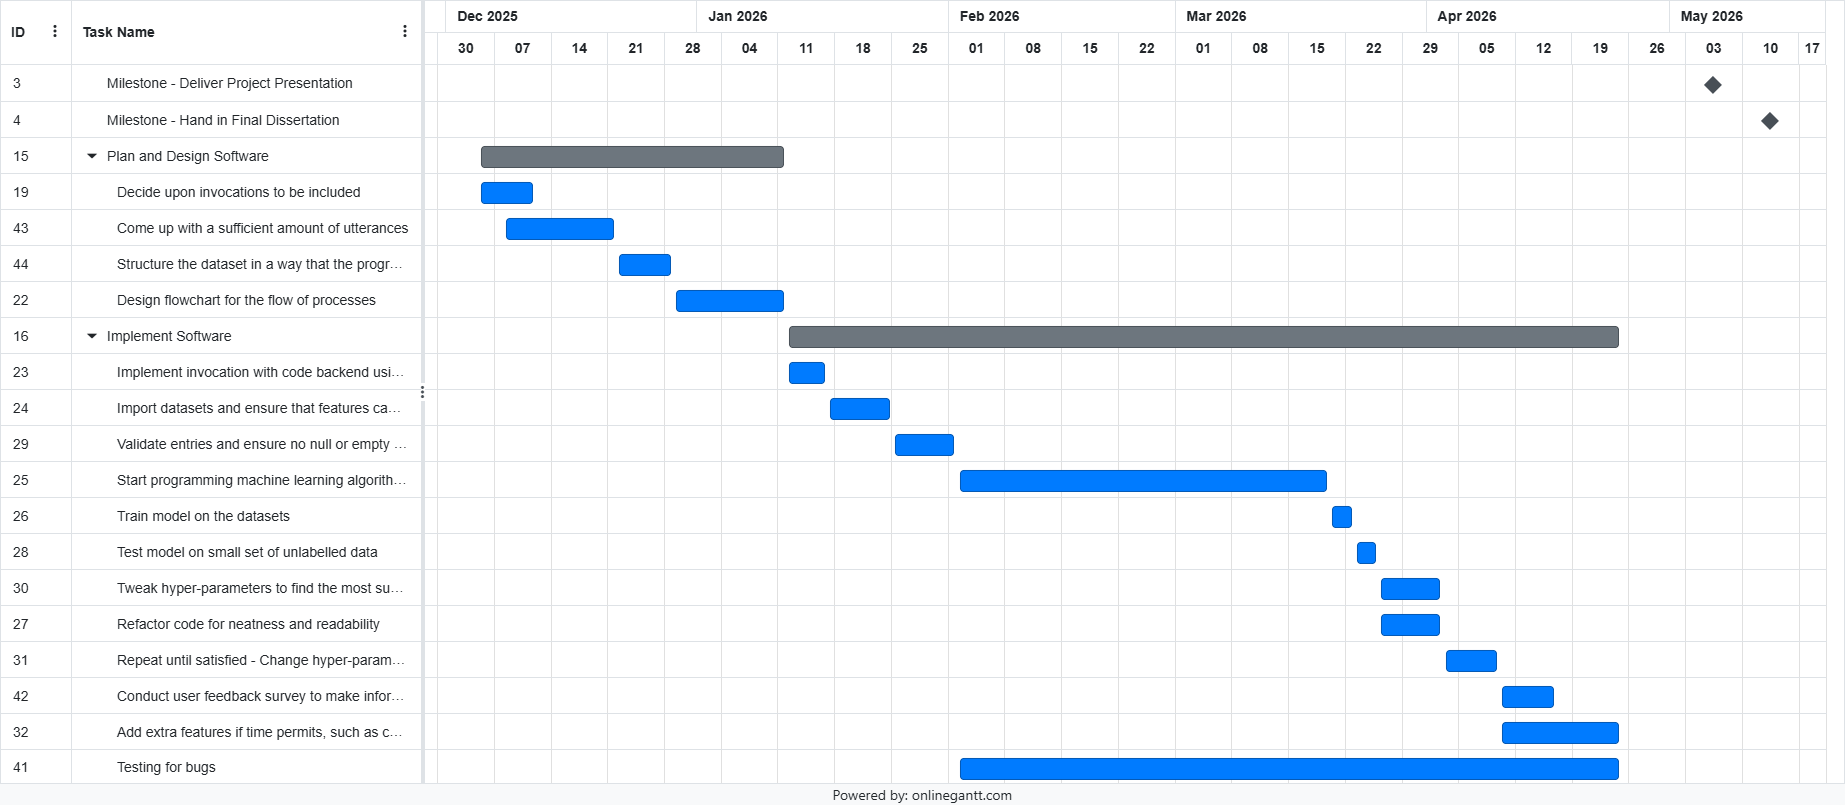
\includegraphics[width=1\linewidth]{./images/Project Plan.png}
    \caption{A Gantt Chart of the Project Plan}
    \label{fig:ProjectGantt}
\end{figure}